%%%%%%%%%%%%%%%%%%%%%%%%%%%%%%%%%%%%%%%%%%%%%%%%%%%%%%%%%
%%             东南大学数电实验报告 LaTeX 模板
%%                SEU-Circuit-Report.cls
%% https://github.com/Teddy-van-Jerry/SEU_Digital_Report
%% ======================================================
%% 版本信息:
%% v1.0 (Nov. 07, 2021)
%% ------------------------------------------------------
%% 模板制作:
%% Teddy van Jerry, (me@teddy-van-jerry.org)
%% * GitHub: https://github.com/Teddy-van-Jerry
%% * Website: https://teddy-van-jerry.org
%% * Blog: https://blog.teddy-van-jerry.org
%% ------------------------------------------------------
%% 使用说明:
%% 1. 编译使用 XeLaTeX 和 Biber
%% 2. 报告基本信息通过修改导言区以 exp 开头的命令
%% 3. 参考文献位于 ref/ref.bib
%% 4. 报告模板依据 MIT License 开源共享
%% ------------------------------------------------------
%% Copyright 2021 (c) Teddy van Jerry
%%
%% Permission is hereby granted, free of charge, to any
%% person obtaining a copy of this software and
%% associated documentation files (the "Software"), to
%% deal in the Software without restriction, including
%% without limitation the rights to use, copy, modify,
%% merge, publish, distribute, sublicense, and/or sell
%% copies of the Software, and to permit persons to whom
%% the Software is furnished to do so, subject to the
%% following conditions:
%%
%% The above copyright notice and this permission notice
%% shall be included in all copies or substantial
%% portions of the Software.
%% 
%% THE SOFTWARE IS PROVIDED "AS IS", WITHOUT WARRANTY OF
%% ANY KIND, EXPRESS OR IMPLIED, INCLUDING BUT NOT
%% LIMITED TO THE WARRANTIES OF MERCHANTABILITY, FITNESS
%% FOR A PARTICULAR PURPOSE AND NONINFRINGEMENT. IN NO
%% EVENT SHALL THE AUTHORS OR COPYRIGHT HOLDERS BE LIABLE
%% FOR ANY CLAIM, DAMAGES OR OTHER LIABILITY, WHETHER IN
%% AN ACTION OF CONTRACT, TORT OR OTHERWISE, ARISING
%% FROM, OUT OF OR IN CONNECTION WITH THE SOFTWARE OR THE
%% USE OR OTHER DEALINGS IN THE SOFTWARE.
%%%%%%%%%%%%%%%%%%%%%%%%%%%%%%%%%%%%%%%%%%%%%%%%%%%%%%%%%%

%% 使用实验报告模板类(字体大小 11pt 约为五号字)
\documentclass[11pt]{SEU-Digital-Report}

%%%%%%%%%%%%%%%%%%%% 报告基本信息 %%%%%%%%%%%%%%%%%%%%
\expno{二} % 实验序号
\expname{组合逻辑与设计} % 实验名称
\expauthor{赵舞穹} % 姓名
\expID{61520522} % 学号
\expmates{郑瑞琪} % 同组
\expmatesID{61520523} % 学号(同组)
\expmajor{工科试验班} % 专业
\explab{计算机硬件技术} % 实验室
\expdate{2021年11月5日} % 实验日期
\expreportdate{\today} % 实验日期
\expgrade{} % 成绩评定
\exptutor{冯熳} % 评阅教师
%%%%%%%%%%%%%%%%%%%%%%%%%%%%%%%%%%%%%%%%%%%%%%%%%%%%

\usepackage{pgfplots}
\pgfplotsset{compat=1.11}

%% 报告正文
\begin{document}
    % 打印封面页
    \exptitlepage

    \tableofcontents
    \newpage

    \section{实验目的与内容}
        
        \begin{enumerate}
            \item 熟进一步熟悉数字逻辑与硬件接口基本实验仪器的使用及TPC 实验装置中基本数字
            逻辑单元的基本原理和组成结构, 学会利用开关输入/LED 发光管/8 段数码管输出电路及示
            波器、电平逻辑笔等验证测试组合逻辑基本特性;
            \item 分析掌握TPC 实验装置板上组合逻辑电路(开关电平转换、LED 发光管驱动、与
            或非门、74LS244 三态总线缓冲器)、扩展CD4518 译码器(BCD-7 段数码管)的工作原理
            和实验方案,完成接线、演示功能及特性验证;
            \item 在认识HDL 和FPGA 设计工具软件基本概念、功能、逻辑设计流程的基础上,学
            习掌握FPGA 数字系统基于门级(原理图)、数据流和行为描述的HDL 模型的基本开发方
            法,通过实践理解开发组合逻辑设计过程;
            \item 完成典型实验电路的HDL 模型搭建、模块编程、配置、调试、分析环节,完成仿
            真运行分析和输入输出演示实验,掌握基于工具软件的组合逻辑设计概念和设计流程.
        \end{enumerate}

    \section{基本实验原理}

            \begin{device}{}{devices}
                \begin{itemize}
                    \item 清华科教仪器厂TPC-ZK-II\_PCI 微机接口实
                    验装置
                    \item EEEC-020A 计算机组成实验箱一台(自带电压表)
                    \item RIGAL DG1022U 25MHz 双路波形发生器
                    \item RIGOL DS1072E-EDU 70MHz 双踪数字记忆示波器
                    \item Xilinx Vivado \textit{HLx} 2017.4
                    \item Ubuntu 20 / Windows 11 (x86\_64){\kaishu\color{gray}(主要实验于 Ubuntu 平台完成)}
                    \item 没有具体的开发板,仅限于线上仿真和使用 Verilog 进行电路设计
                \end{itemize}
            \end{device}

        \subsection{三态总线缓冲器特性实验}

            \subsubsection{简单组合逻辑}

                利用与门、或门和非门搭建图~\ref{fig:1_circuit}~组合逻辑电路,输入接开关,输出接指示灯.
                $in=000\sim 111$.

                \begin{figure}[htbp]
                    \centering
                    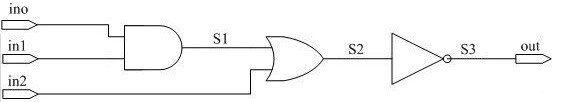
\includegraphics[width=.5\linewidth]{fig/简单组合逻辑电路.jpg}
                    \caption{简单组合逻辑电路特性\cite{guide}}
                    \label{fig:1_circuit}
                \end{figure}

                通过理论分析,可以得到其真值表如表~\ref{tab:1_truth_table}~所示.

                \begin{table}[htbp]
                    \centering
                    \begin{tabular}{ccc|ccc|c}
                        \toprule
                        $in_0$ & $in_1$ & $in_2$ & $S_1$ & $S_2$ & $S_3$ & $out$ \\
                        \midrule
                        0 & 0 & 0 & 0 & 0 & 1 & 1 \\
                        0 & 0 & 1 & 0 & 1 & 0 & 0 \\
                        0 & 1 & 0 & 0 & 0 & 1 & 1 \\
                        0 & 1 & 1 & 0 & 1 & 0 & 0 \\
                        1 & 0 & 0 & 0 & 0 & 1 & 1 \\
                        1 & 0 & 1 & 0 & 1 & 0 & 0 \\
                        1 & 1 & 0 & 1 & 1 & 0 & 0 \\
                        1 & 1 & 1 & 1 & 1 & 0 & 0 \\
                        \bottomrule
                    \end{tabular}
                    \caption{简单组合逻辑电路的真值表}
                    \label{tab:1_truth_table}
                \end{table}

                我们也可以写出其布尔表达式:
                \begin{equation}\label{eq:1_logic}
                    out=\overline{(in_0\times in_1)+in_2}=(\overline{in_0}+\overline{in_1})\overline{in_2}.
                \end{equation}

            \subsubsection{三态总线缓冲器}

                三台总线缓存器相当于三态门(three-state logic)的叠加,
                三态门的主要情况如下\cite{wiki:3logic}:

                In digital electronics three-state, tri-state, or 3-state logic allows an output or input pin/pad to assume a high impedance state, effectively removing the output from the circuit, in addition to the 0 and 1 logic levels.

                This allows multiple circuits to share the same output line or lines (such as a bus which cannot listen to more than one device at a time).
                
                Three-state outputs are implemented in many registers, bus drivers, and flip-flops in the 7400 and 4000 series as well as in other types, but also internally in many integrated circuits. Other typical uses are internal and external buses in microprocessors, computer memory, and peripherals. Many devices are controlled by an active-low input called OE (Output Enable) which dictates whether the outputs should be held in a high-impedance state or drive their respective loads (to either 0- or 1-level).

                \begin{figure}[htbp]
                    \centering
                    \subfloat[电路图]{
                        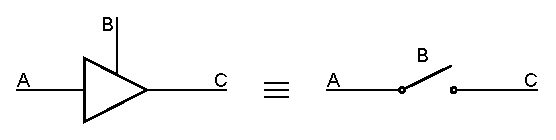
\includegraphics[width=.5\linewidth]{fig/three-logic.eps}
                        \label{subfig:3logic_circuit}
                    }\qquad
                    \subfloat[真值表]{
                        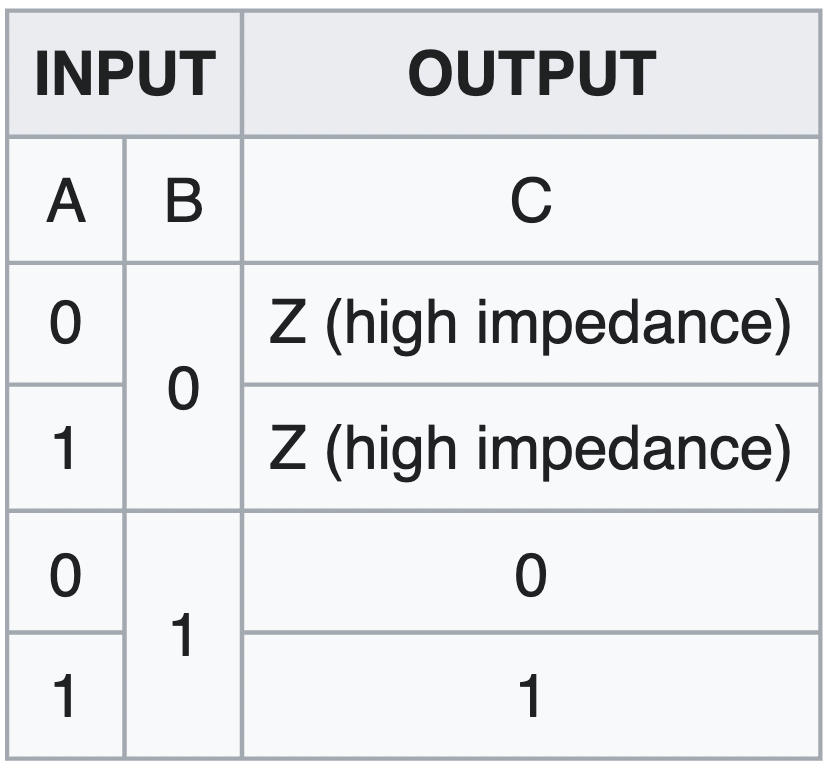
\includegraphics[width=.2\linewidth]{fig/three-logic-truth-table.png}
                        %\label{}
                    }
                    \caption{三态门\cite{wiki:3logic}}
                    \label{fig:3logic}
                \end{figure}

            完整的三态总线驱动器见图~\ref{subfig:3logic_all}.

        \newpage

        \subsection{扩展CD4518 译码器(BCD-7 段数码管)应用}

            CD4511BC 是一BCD-7 段数码管的译码驱动器, 引脚功能如图~\ref{fig:BCD-7},真值表如图~\ref{fig:BCD-7-truth-table}.

            \begin{figure}[htbp]
                \centering
                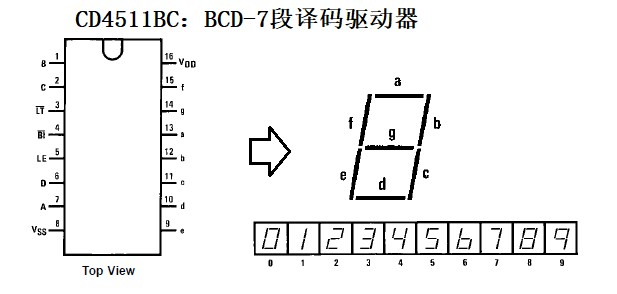
\includegraphics[width=.6\linewidth]{fig/BCD-7.jpg}
                \caption{CD4511 BCD-7 段显示译码驱动器\cite{guide}}
                \label{fig:BCD-7}
            \end{figure}
            \begin{figure}[htbp]
                \centering
                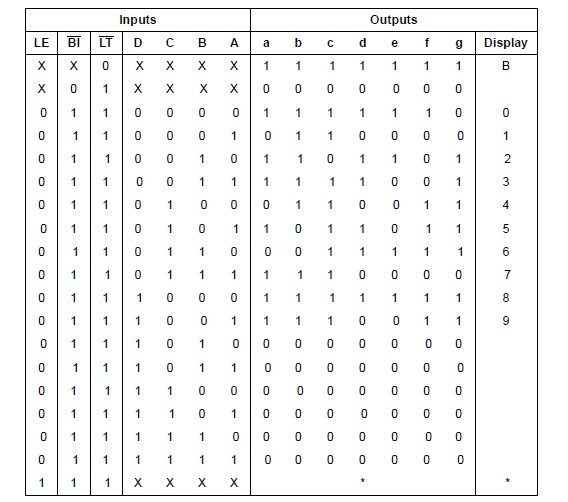
\includegraphics[width=.7\linewidth]{fig/BCD-7-truth-table.jpg}
                \caption{CD4511 BCD-7 段显示译码驱动器真值表\cite{guide}}
                \label{fig:BCD-7-truth-table}
            \end{figure}

            我们可以给出其逻辑表达式:
            \begin{equation}\label{eq:CD4511_logic}
                \left\{
                    \begin{aligned}
                        a & =\ \sum m(0, 2, 3, 5, 7, 8, 9) &&=\ D+AB+AC+\widebar{A}\widebar{C} \\
                        b & =\ \sum m(0, 1, 2, 3, 4, 7, 8, 9) &&=\ D+\widebar{C}+AB+\widebar{A}\widebar{B} \\
                        c & =\ \sum m(0, 1, 3, 4, 5, 6, 7, 8, 9) &&=\ D+\widebar{B}+A \\
                        d & =\ \sum m(0, 2, 3, 5, 6, 8) &&=\ B+\widebar{A}\widebar{C} \\
                        e & =\ \sum m(0, 2, 6, 8) &&=\ \widebar{A}\widebar{D} \\
                        f & =\ \sum m(0, 4, 5, 6, 8, 9) &&=\ \widebar{A}\widebar{B}+\widebar{B}C+\widebar{B}D+\widebar{A}C \\
                        g & =\ \sum m(2, 3, 4, 5, 6, 8, 9) &&=\ D+AC+B\widebar{C}+\widebar{B}C \\
                    \end{aligned}
                \right.
            \end{equation}
            式中从最小项表达式化为逻辑表达式使用卡诺图(注意有 $d(10,11,12,13,14,15)$).
        
    \section{实验内容}\label{sec:exp}

        \subsection{三态总线缓冲器特性实验}

            \subsubsection{简单组合逻辑}

                利用实验箱上与门、或门和非门搭建图~\ref{fig:1_circuit}~组合逻辑电路,输入接开关,输出接指示灯.
                $in=000\sim 111$.
                真实电路如图~\ref{fig:1_real}~所示.

                \begin{figure}[htbp]
                    \centering
                    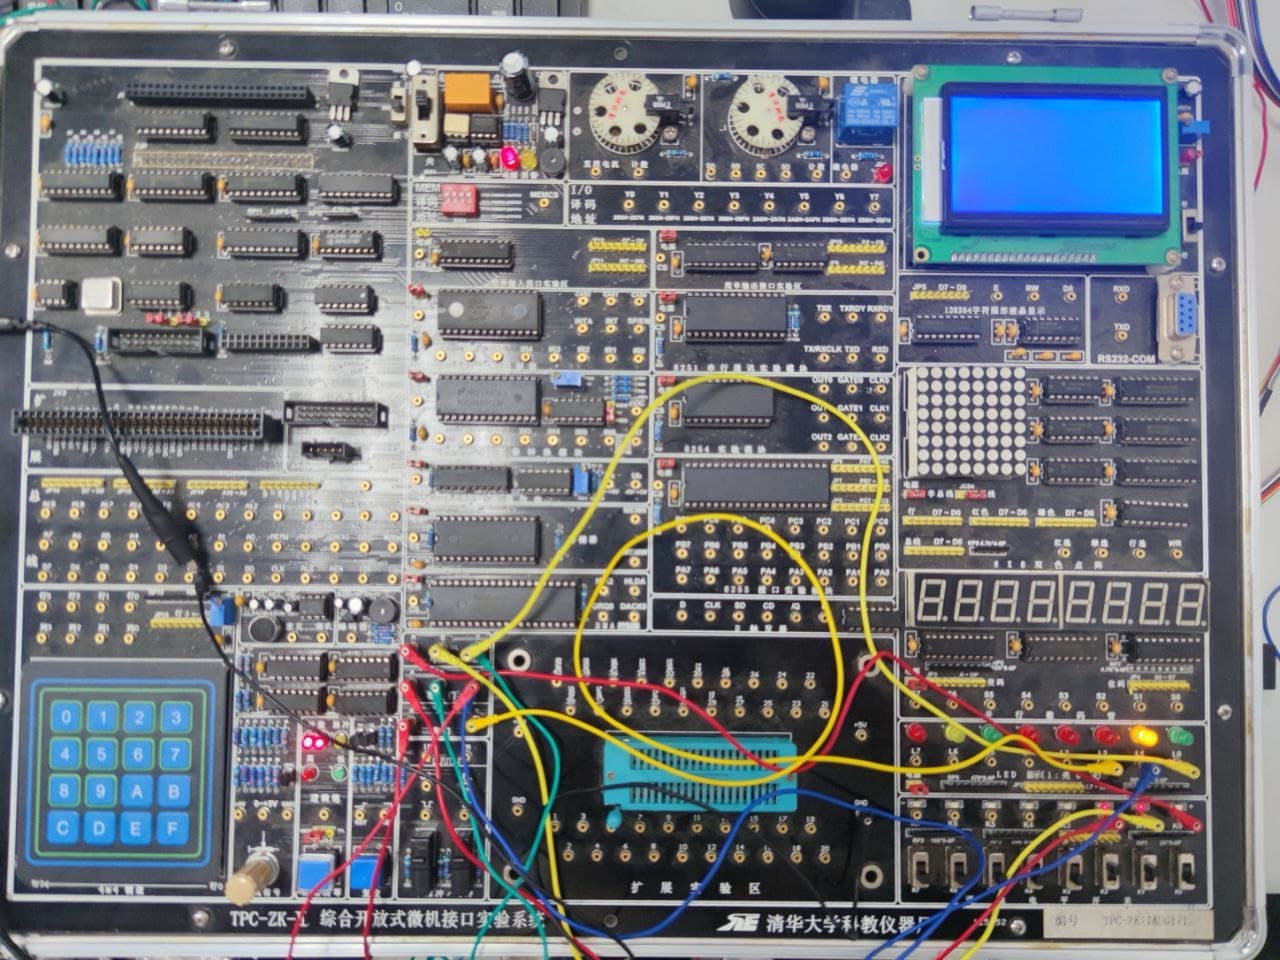
\includegraphics[width=.5\linewidth]{fig/简单组合逻辑真实.jpg}
                    \caption{简单组合逻辑的真实电路连接}
                    \label{fig:1_real}
                \end{figure}

                \begin{note}{示波器的使用}{}
                    注意示波器需要和实验箱共地,否则无法测出实际有效的波形.
                \end{note}

                \begin{analyze}{}{}
                    通过观测示波器高低电平判断以及LED灯的现实,我们发现结果与表~\ref{tab:1_truth_table}~一致,验证了简单组合逻辑电路.
                \end{analyze}

            \subsubsection{三态总线缓冲器}

            接线如图~\ref{fig:exp_3logic},利用实验箱简单输入接口实验区的三态总线缓冲器74LS244(实际为双
            向缓冲器74LS245 单向模式工作,即DIR 接高电平,A$\rightarrow$B).接线:
            \begin{note}{}{}
                期间需要断开PC 机总线.
            \end{note}
            排线1 一端接逻辑开关输入JP1(K0-K7),一端接总线缓冲器输入端JP11(IN7---IN0);

            排线2 一端接总线缓冲器输出/JP12(O7---O0),一端接LED 指示灯显示/JP2(L7---L0).

            按动开关K7 控制使能端,记录示波器观察缓冲器输出(L7-L0)及指示灯状态等结果;

            \begin{figure}[htbp]
                \centering
                \subfloat[原理图]{
                    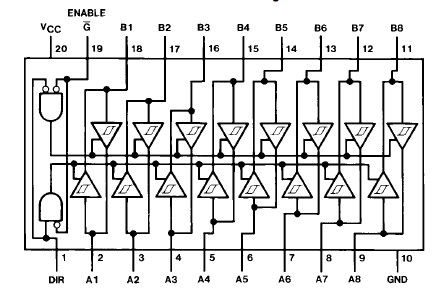
\includegraphics[width=.5\linewidth]{fig/三总线2.jpg}
                    \label{subfig:3logic_all}
                }\qquad
                \subfloat[接线图]{
                    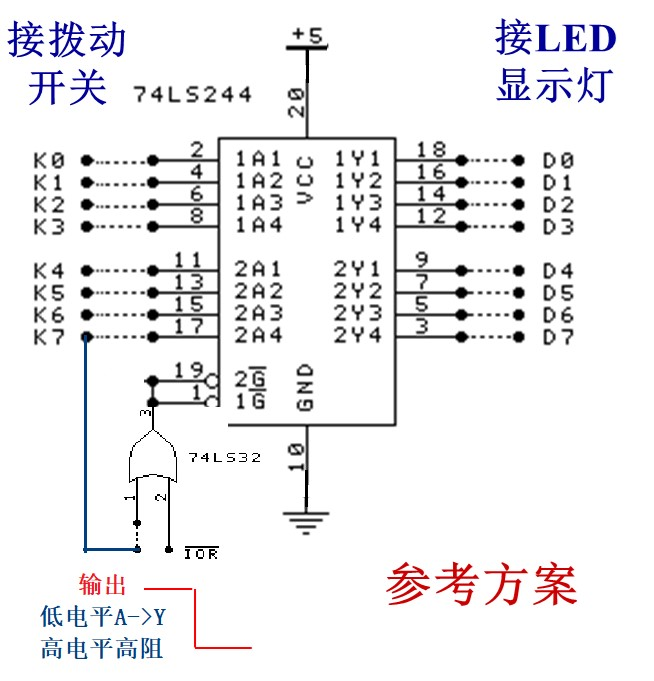
\includegraphics[width=.32\linewidth]{fig/三总线1.jpg}
                    %\label{}
                }
                \caption{8 路三态总线驱动器特性\cite{guide}}
                \label{fig:exp_3logic}
            \end{figure}

            \begin{figure}[htbp]
                \centering
                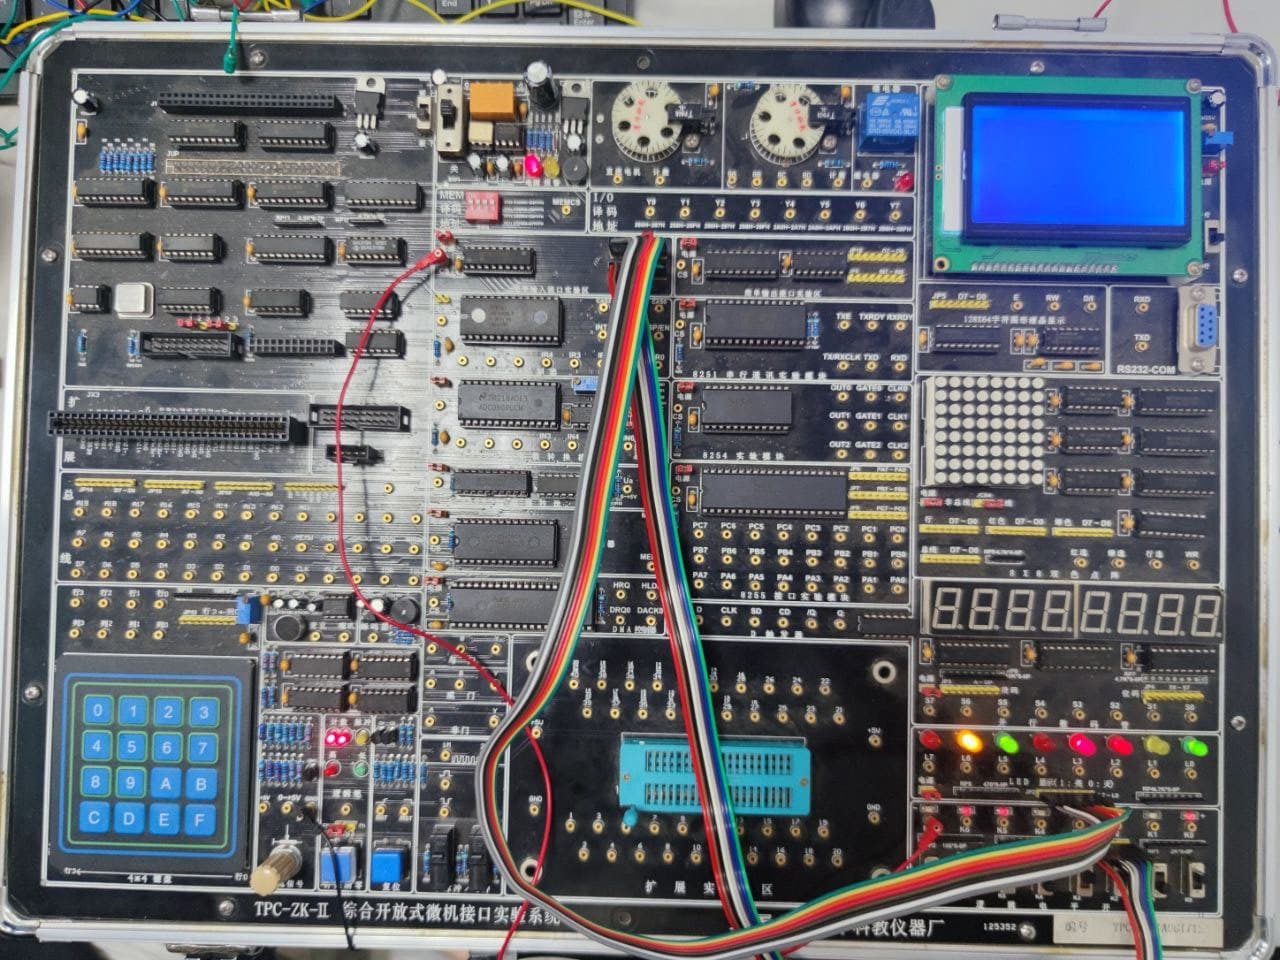
\includegraphics[width=.5\linewidth]{fig/3logic_real.jpg}
                \caption{8 路三态总线驱动器的真实电路连接}
                \label{fig:3logic_real}
            \end{figure}

            \begin{analyze}{}{}
                没有触发时,指示灯不变;经过触发,可以显示触发前对应开关的取值.
            \end{analyze}

        \subsection{扩展CD4518 译码器(BCD-7 段数码管)应用}\label{subsec:4518}
            
            在实验箱扩展实验区顶头插入CD4511 芯片,引脚Pin16-Vcc($+5\mathrm{V}$),Pin8-GND;引
            脚Pin(6) D、(2)C、(1)B、(7)A 分别接开关K3-K0;引脚Pin(5) LE 接低电平,引脚Pin(4) BI
            和(3)LT 接高电平.引脚Pin(9-15) a-g 分别接数码管段选JP3(A---DP)(可借用8255 的PA
            排线与插孔PA0-PA6 过渡,如图1-7).带显示LED 数码管位选$S_x$($x=0\sim7$)接高电平.

            利用8421 开关K3-K0 拨码输入\texttt{0000-1001B}.

            \begin{figure}[htbp]
                \centering
                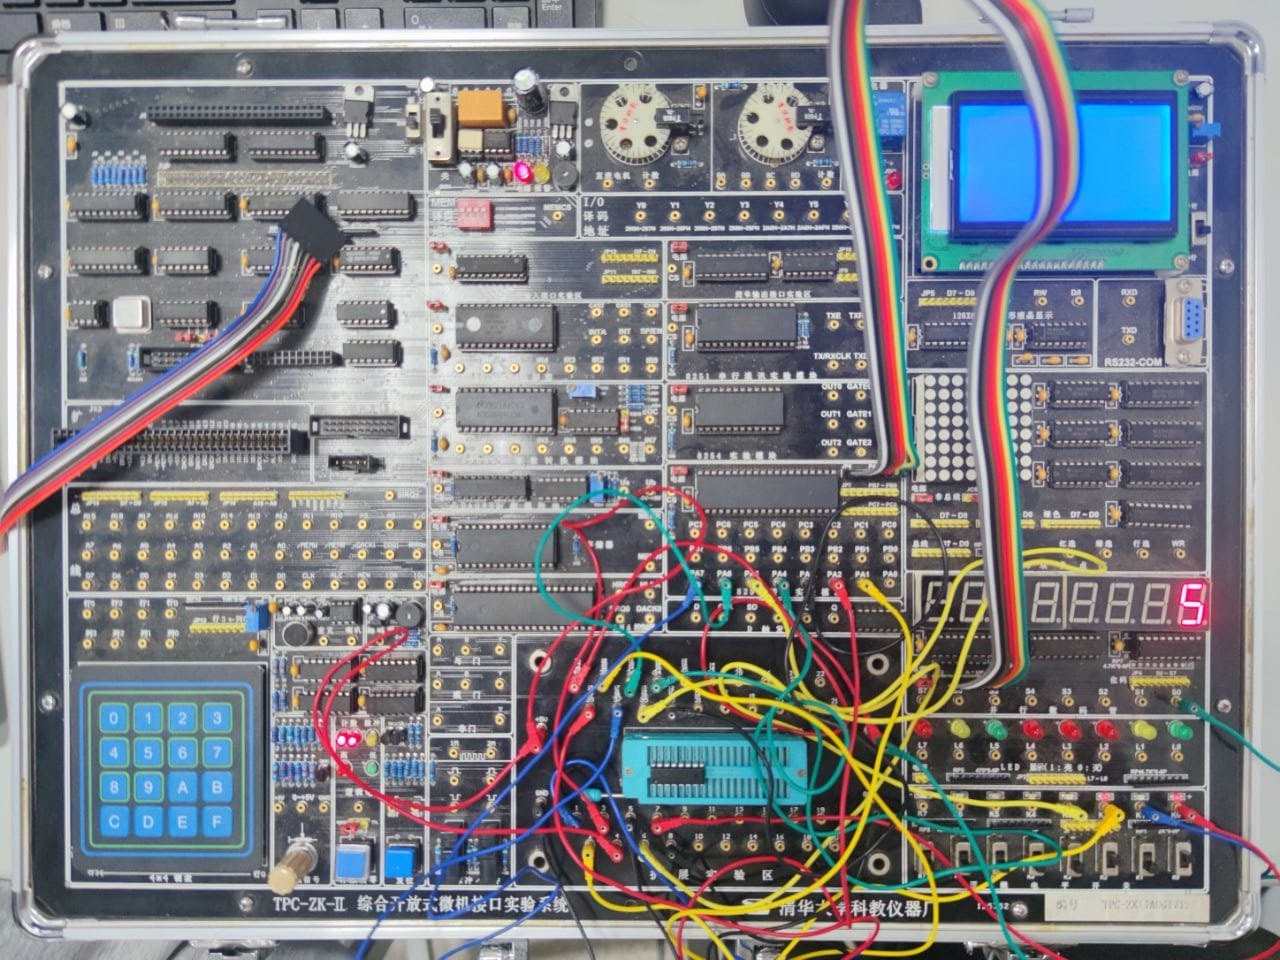
\includegraphics[width=.5\linewidth]{fig/BCD-7-real.jpg}
                \caption{CD4511 BCD-7 段显示译码实际电路}
                \label{fig:bcd7_real}
            \end{figure}

            \begin{analyze}{}{}
                通过控制 开关K3-K0 作为输入的 8421 码,成功显示数字,并且与图~\ref{fig:BCD-7-truth-table}~中的结果一致.
            \end{analyze}

        \subsection{CAD 逻辑设计与仿真}

            \subsubsection{三级组合逻辑电路}

                利用门级模型,搭建图~\ref{fig:1_circuit}~电路,按真值表模拟输入,完成仿真分析和特性记录;
                改变门延时参数,观察记录状态变化.

                \begin{lstlisting}[language=verilog, title=cl01\_tb.v]
module cl01_tb(input [2:0] in, output out1); // testbench file
  reg [2:0] xin; 
  wire out; 
  wire [2:0] s; 
  cl01 DUT(.in(xin),.S1(s[0]),.S2(s[1]), .S3(s[2]), .out(out)); 

assign out1=out; 
initial 
  begin 
    #10 xin = 0; 
    #10 xin = 1; 
    #10 xin = 2; 
    #10 xin = 3; 
    #10 xin = 4; 
    #10 xin = 5; 
    #10 xin = 6; 
    #10 xin = 7; 
    #10 xin = 0; 
    #10; 
  end
endmodule
                \end{lstlisting}
                \begin{lstlisting}[language=verilog, title=cl01.v]
`timescale 1ns / 100ps 
module cl01( 
  input [2:0] in, 
  output S1,S2,S3, 
  output out 
); // GATE model
  // wire S0,S1,S2,S3; 
  and #1 U1(S1,in[0],in[1]); 
  or  #2 U2(S2,S1,in[2]); 
  not #3 U3(S3,S2); 
  assign out=S3;
endmodule
                \end{lstlisting}

                \begin{analyze}{}{}
                行为仿真(图~\ref{fig:vivado_1_simu},\texttt{behavioral simulation})的结果与表~\ref{tab:1_truth_table}~一致,不过需要注意表~\ref{tab:1_truth_table}~中 $in$ 和 $S$ 的顺序是反的.

                RTL 门级电路结果(图~\ref{fig:vivado_1_RTL})与设计(图~\ref{fig:1_circuit})一样,此处代码采用了门级描述,其实也可以使用行为描述,如下代码:
                \begin{lstlisting}[language=verilog, title=cl01.v, numbers=none, backgroundcolor=\color{green!3}]
`timescale 1ns / 100ps 
module cl01( 
  input [2:0] in,
  output S1,S2,S3,
  output out
  ); // BEHAVIORAL model
  // wire S0,S1,S2,S3;
  assign S1=in[0]&in[1];
  assign S2=S1|in[2];
  assign S3=~S2;
endmodule
                \end{lstlisting}

                此外,修改门延时影响不大,就是各输出变化的延迟变长了,和预期一致.
            \end{analyze}

                \begin{figure}[htbp]
                    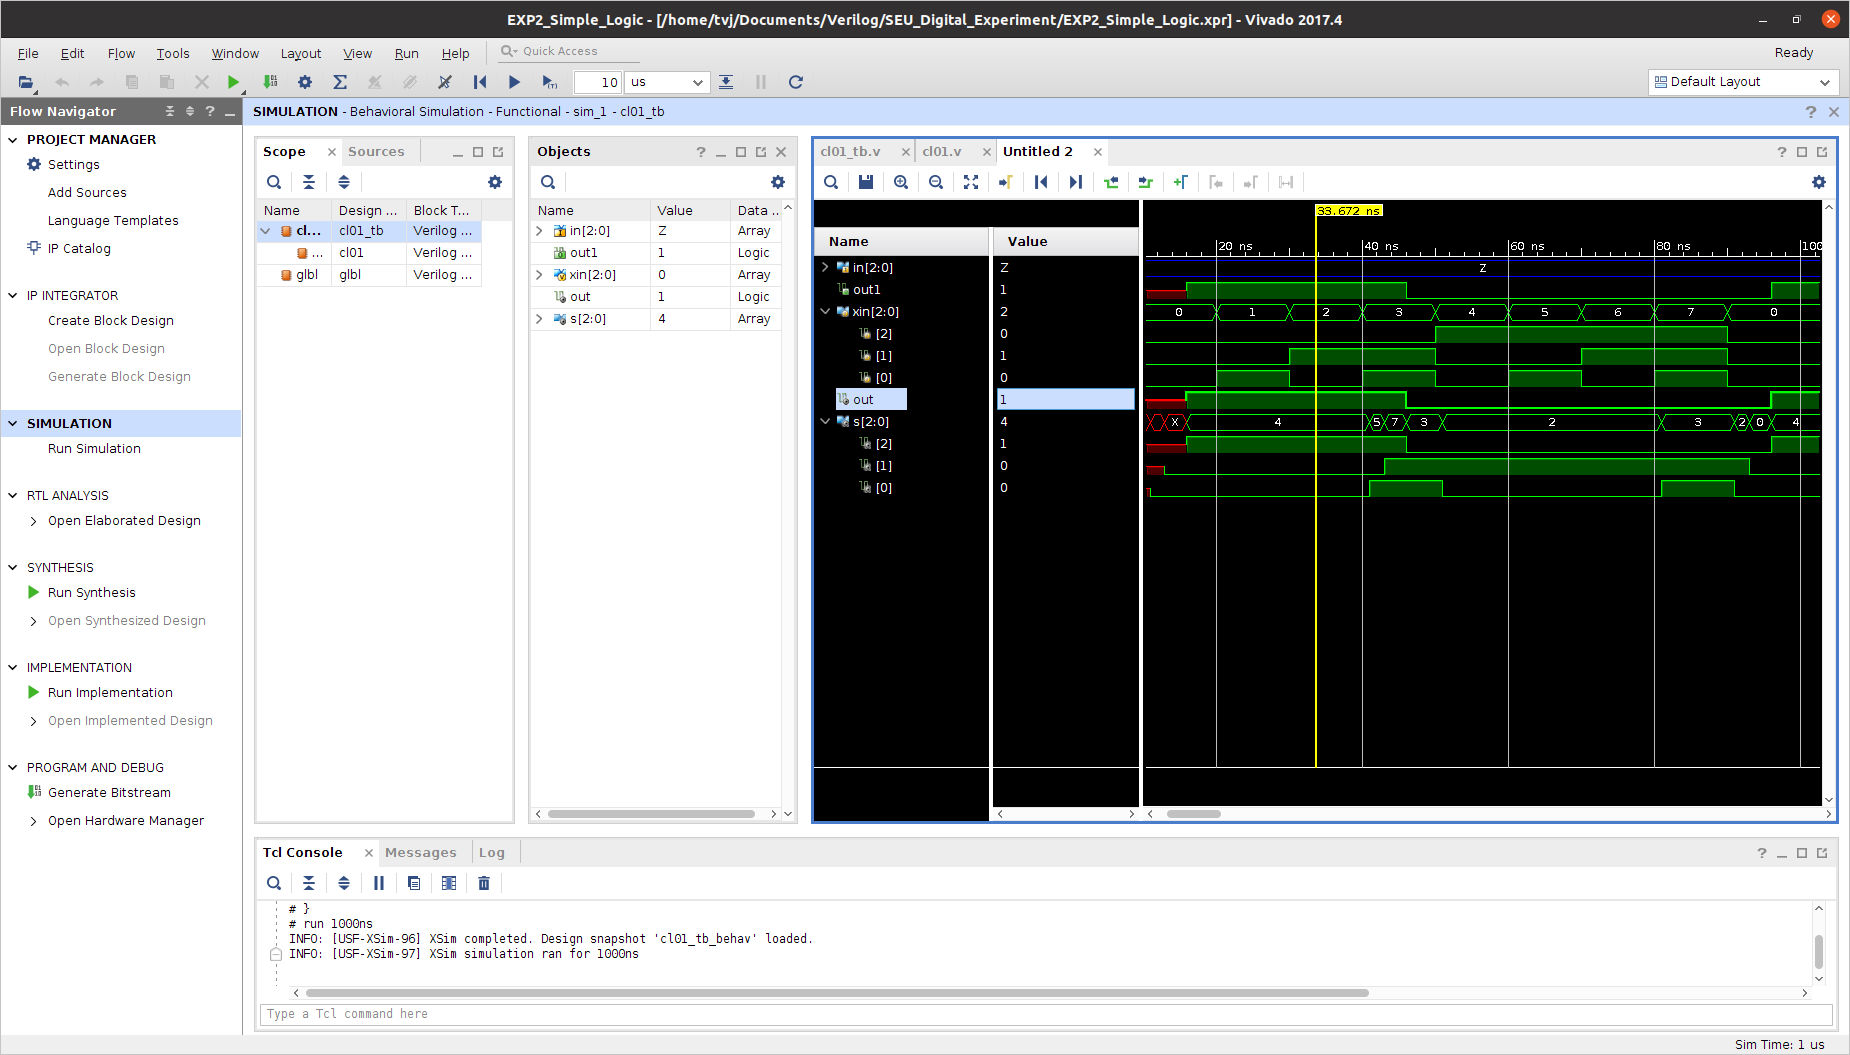
\includegraphics[width=\linewidth]{fig/vivado/1_simu.png}
                    \caption{三级组合逻辑电路的行为仿真}
                    \label{fig:vivado_1_simu}
                \end{figure}

                \begin{figure}[htbp]
                    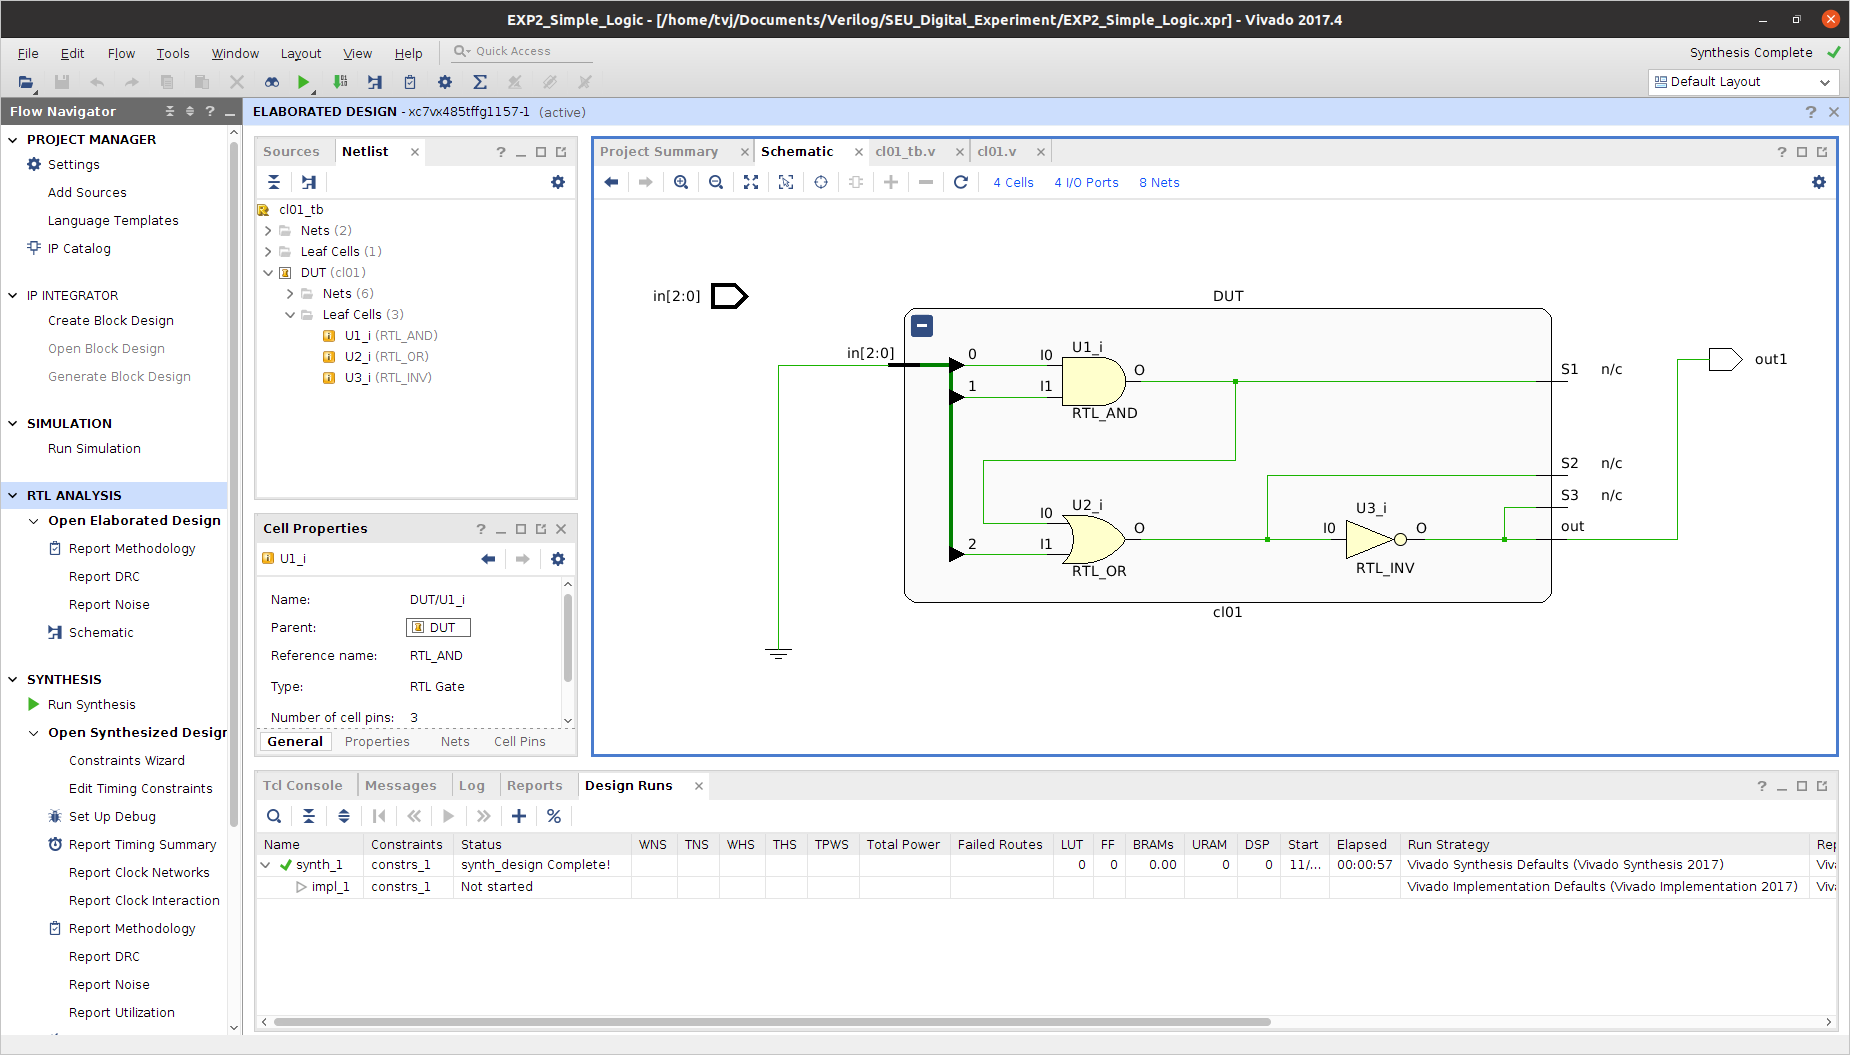
\includegraphics[width=\linewidth]{fig/vivado/1_RTL.png}
                    \caption{三级组合逻辑电路的RTL级电路}
                    \label{fig:vivado_1_RTL}
                \end{figure}


            \newpage

            \subsubsection{搭建3-8 译码器}

                仿74LS138 结构和功能,搭建3-8
                译码器数据流模型.

                \begin{figure}[htbp]
                    \centering
                    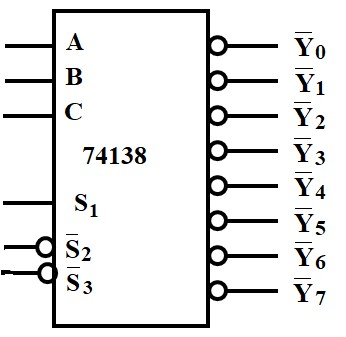
\includegraphics[width=.25\linewidth]{fig/74138.jpg}
                    \caption{74138模块\cite{guide}}
                    \label{fig:74138}
                \end{figure}

                \begin{lstlisting}[language=verilog, title=x74x138\_tb.v]
module x74x138_tb; // testbench file
  reg g1; 
  reg g2; 
  reg g3; 
  reg [2:0] a; 
  wire [7:0] y; 
 
  x74x138 u1(g1,g2,g3,a,y); 
  initial begin 
    g1=0; 
    g2=0; 
    g3=0; 
    a =0; 
    #100;
    g1=1; 
    g2=0; 
    g3=0; 
  end 
  always #100 a=a+1; // clock signal
endmodule
                \end{lstlisting}
                \begin{lstlisting}[language=verilog, title=x74x138.v]
module x74x138(g1,g2,g3,a,y); // define model for 74138
input g1,g2,g3; 
input [2:0] a; 
output [7:0] y; // declare output variable
reg [7:0] y=0; // in declaration it should be 'reg'
 
  always @ * 
  begin 
    if(g1 && ~g2 && ~g3) // gate terminal
      case(a) 
      7: y = 8'b01111111; 
      6: y = 8'b10111111; 
      5: y = 8'b11011111; 
      4: y = 8'b11101111; 
      3: y = 8'b11110111; 
      2: y = 8'b11111011; 
      1: y = 8'b11111101; 
      0: y = 8'b11111110; 
      default: y= 8'b11111111; 
      endcase 
    else 
    y = 8'b11111111; 
  end 
endmodule
                \end{lstlisting}

            \begin{analyze}{}{}
                如图~\ref{fig:vivado_2_simu}~所示行为仿真结果显示3-8译码器工作正常,此外,RTL级电路(图~\ref{fig:vivado_2_simu})让我对 74138 有了更深入的了解.

                这个代码中是没有门延时的,所以时间点对的非常准.
            \end{analyze}

            \begin{figure}[htbp]
                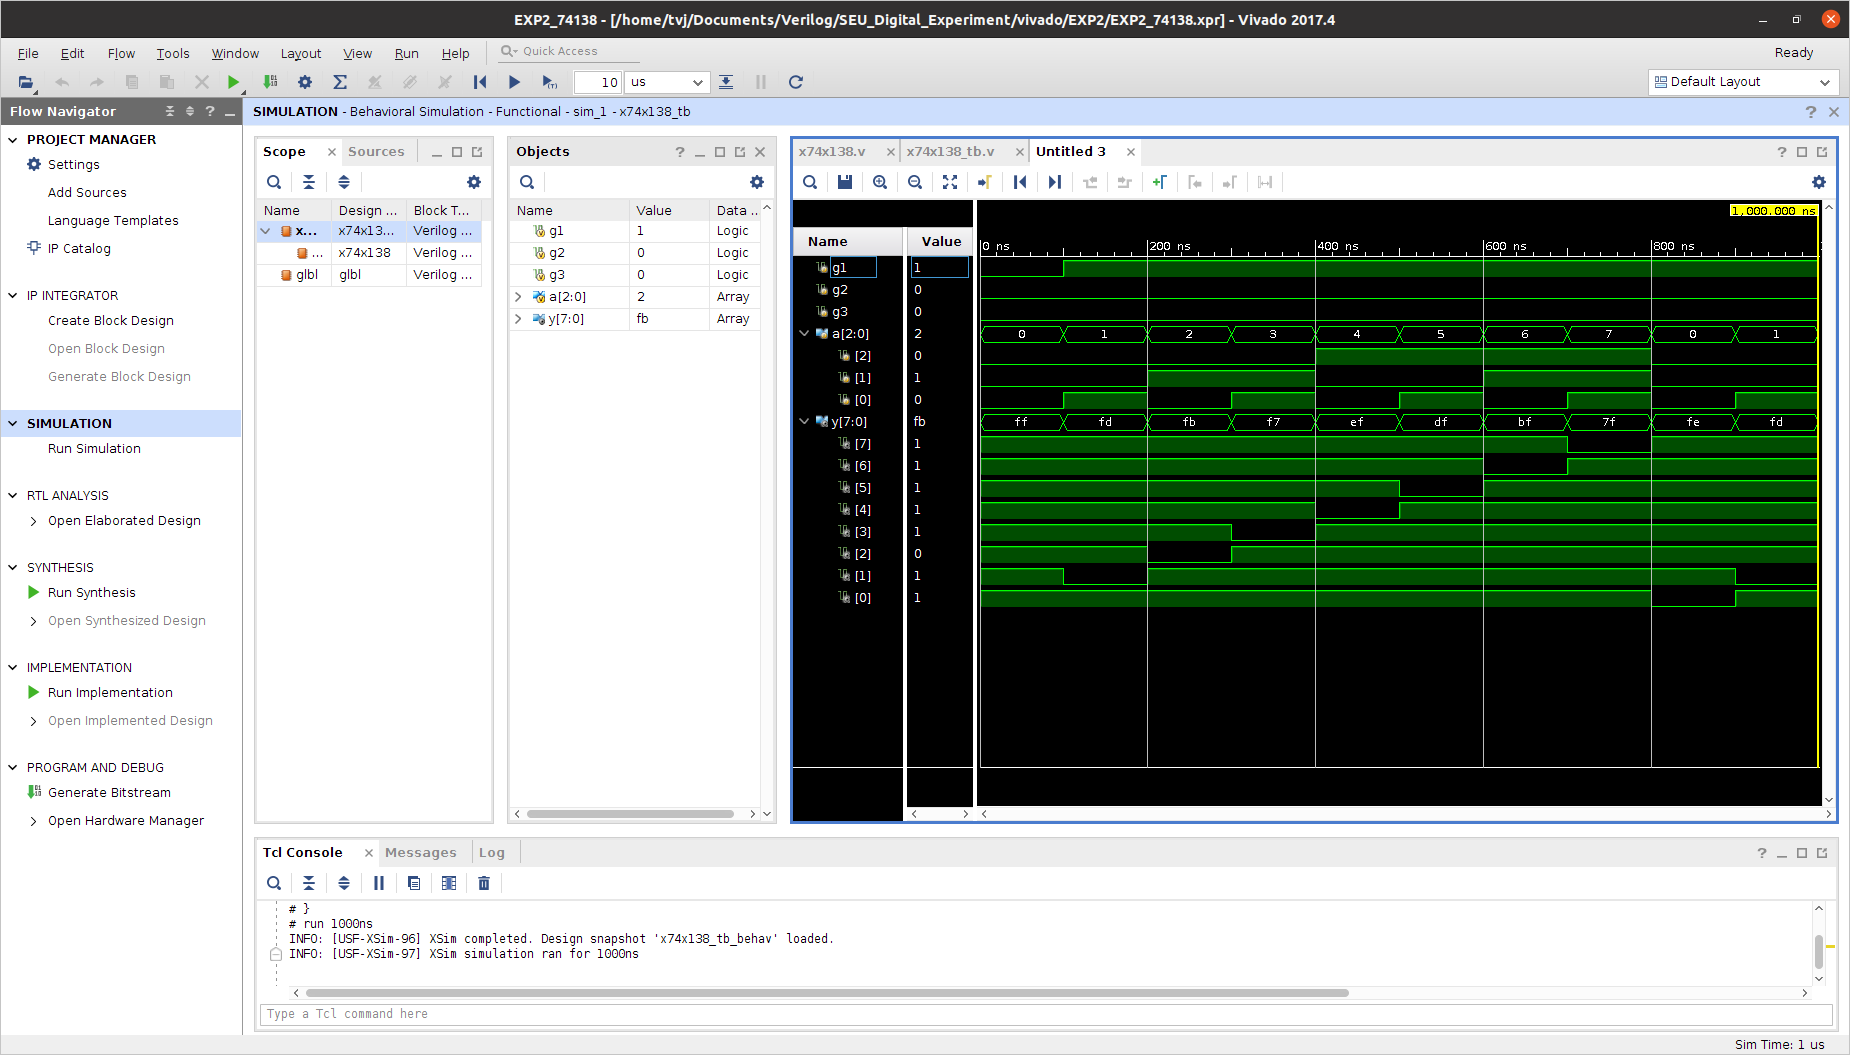
\includegraphics[width=\linewidth]{fig/vivado/2_simu.png}
                \caption{74138的行为仿真}
                \label{fig:vivado_2_simu}
            \end{figure}

            \begin{figure}[htbp]
                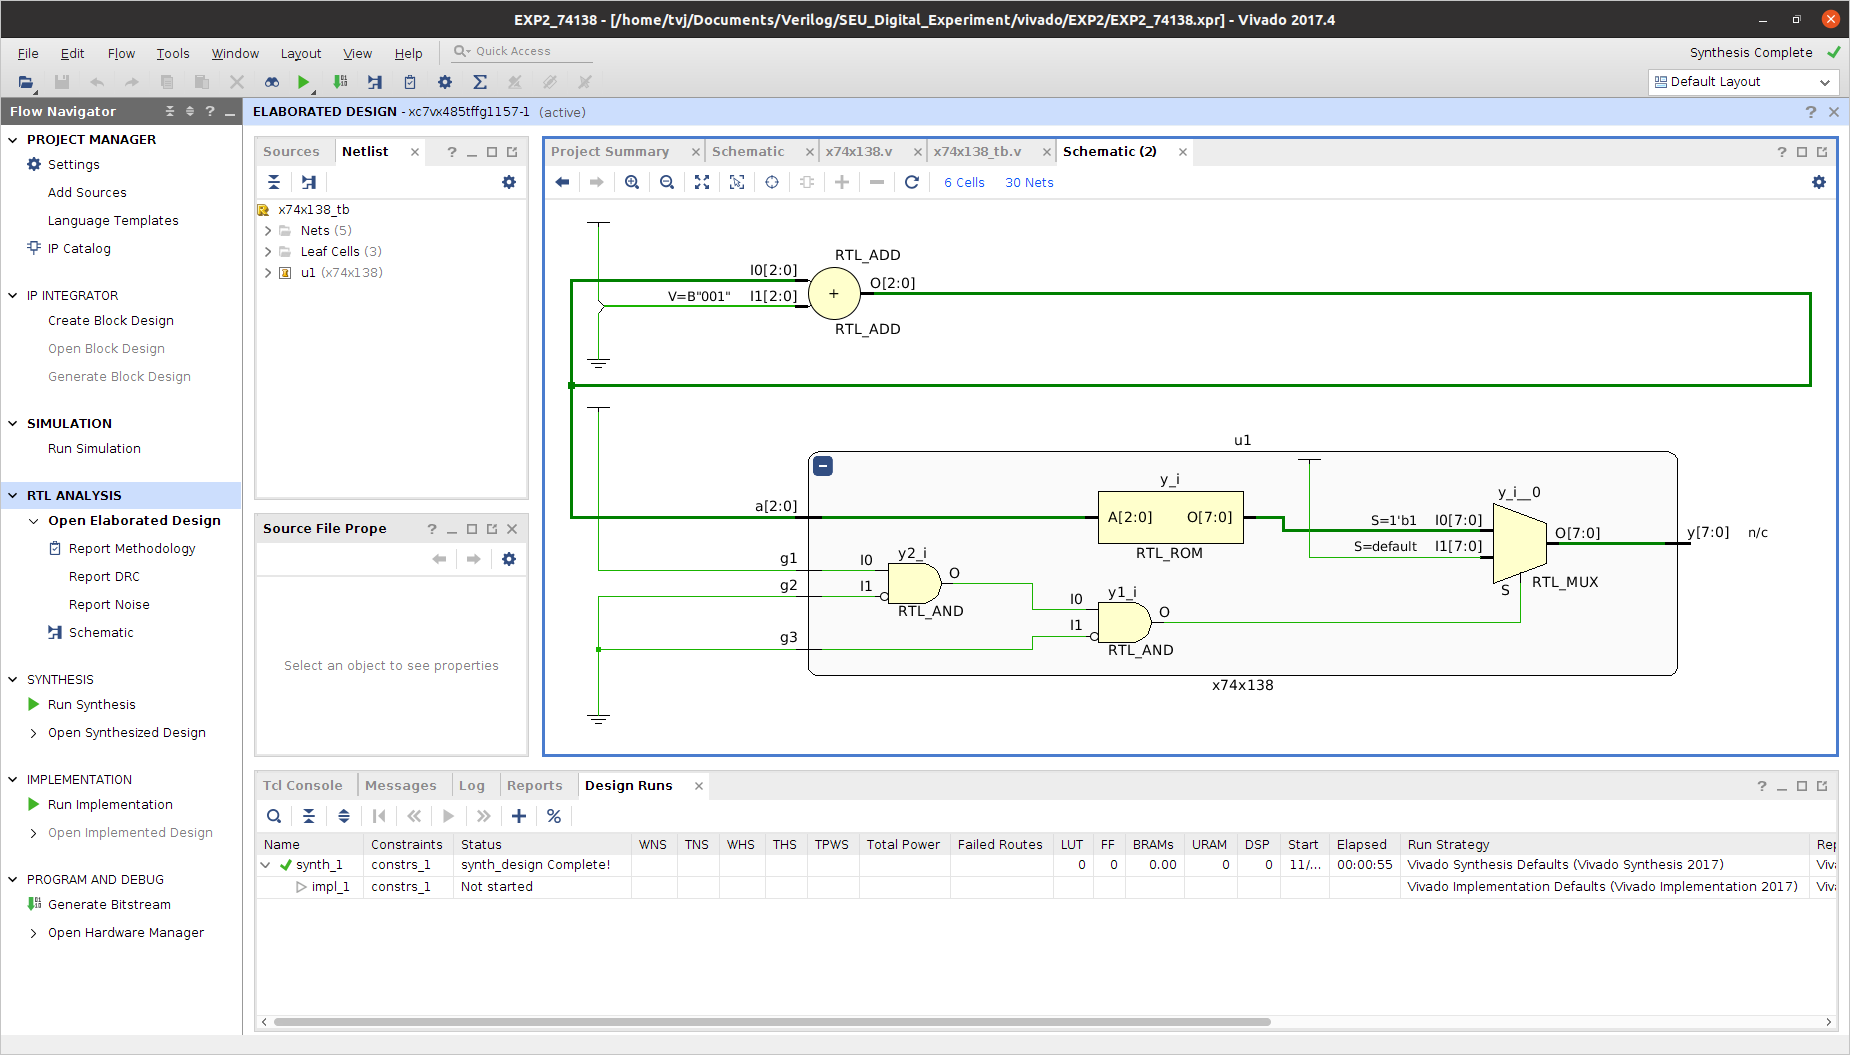
\includegraphics[width=\linewidth]{fig/vivado/2_RTL.png}
                \caption{74138的RTL级电路}
                \label{fig:vivado_2_RTL}
            \end{figure}

            \newpage
            \subsubsection{搭建BCD-7 段译码驱动器数据流模型}

                参考第~\ref{sec:exp}.\ref{subsec:4518}~节,参考CD4511 结构和功能,搭建BCD-7 段译码驱动器数据流模型.

                \begin{lstlisting}[language=verilog, title=CD4511\_tb.v]
module CD4511_tb;

  wire a_tb, b_tb, c_tb, d_tb, e_tb, f_tb, g_tb;
  reg D_tb, C_tb, B_tb, A_tb;
  reg LTbarr_tb, BIbarr_tb, LE_tb;
  
  CD4511 dut( a_tb, b_tb, c_tb, d_tb, e_tb, f_tb, g_tb, D_tb, C_tb, B_tb, A_tb, LTbarr_tb, BIbarr_tb, LE_tb );

  initial
  begin
    LTbarr_tb = 0; #1
    LTbarr_tb = 1; BIbarr_tb = 0; #1
    LTbarr_tb = 1; BIbarr_tb = 1; LE_tb = 0; 
    D_tb = 0; C_tb = 0; B_tb = 0; A_tb = 0; #1
    D_tb = 0; C_tb = 0; B_tb = 0; A_tb = 1; #1
    D_tb = 0; C_tb = 0; B_tb = 1; A_tb = 0; #1
    D_tb = 0; C_tb = 0; B_tb = 1; A_tb = 1; #1
    D_tb = 0; C_tb = 1; B_tb = 0; A_tb = 0; #1
    D_tb = 0; C_tb = 1; B_tb = 0; A_tb = 1; #1
    D_tb = 0; C_tb = 1; B_tb = 1; A_tb = 0; #1
    D_tb = 0; C_tb = 1; B_tb = 1; A_tb = 1; #1
    D_tb = 1; C_tb = 0; B_tb = 0; A_tb = 0; #1
    D_tb = 1; C_tb = 0; B_tb = 0; A_tb = 1; #1
    D_tb = 1; C_tb = 0; B_tb = 1; A_tb = 0; #1
    D_tb = 1; C_tb = 0; B_tb = 1; A_tb = 1; #1
    D_tb = 1; C_tb = 1; B_tb = 0; A_tb = 0; #1
    D_tb = 1; C_tb = 1; B_tb = 0; A_tb = 1; #1
    D_tb = 1; C_tb = 1; B_tb = 1; A_tb = 0; #1
    D_tb = 1; C_tb = 1; B_tb = 1; A_tb = 1; #1;
  end
endmodule

/* Reference:
https://www.embarcados.com.br/
tutorial-de-verilog-conversor-bcd-para-7-segmentos/
*/
                \end{lstlisting}
                \begin{lstlisting}[language=verilog, title=CD4511.v]
module CD4511( a, b, c, d, e, f, g, D, C, B, A , LTbarr, BIbarr, LE ); // BCD -> 7 segments

output a, b, c, d, e, f, g;
input D, C, B, A;
input LTbarr, BIbarr, LE;
reg  [6:0] SevenSegments;

always @(*)

if ( LTbarr == 0 )
begin
    SevenSegments = 8'b11111111;  
end
else 
begin
  if ( BIbarr == 0 )
  begin
    SevenSegments = 8'b00000000;  
  end
  else if(( BIbarr == 1 ) && ( LTbarr == 1 ) && ( LE == 0))
  begin
    case({D, C, B, A})
      4'b0000: SevenSegments = 7'b1111110;
      4'b0001: SevenSegments = 7'b0110000;
      4'b0010: SevenSegments = 7'b1101101;
      4'b0011: SevenSegments = 7'b1111001;
      4'b0100: SevenSegments = 7'b0110011;
      4'b0101: SevenSegments = 7'b1011011;
      4'b0110: SevenSegments = 7'b0011111;
      4'b0111: SevenSegments = 7'b1110000;
      4'b1000: SevenSegments = 7'b1111111;
      4'b1001: SevenSegments = 7'b1110011;
      default: SevenSegments = 7'b0000000;
    endcase
  end
end

assign {a, b, c, d, e, f, g} = SevenSegments;

endmodule

/* Reference:
https://www.embarcados.com.br/
tutorial-de-verilog-conversor-bcd-para-7-segmentos/
*/
                \end{lstlisting}

                \begin{analyze}{}{}
                    CD4511 代码的总体思路较为清晰,
                    即在某一个特定输入下时某几根LED管需要亮起.
                    因此,公式~\eqref{eq:CD4511_logic}~其实不需要进行推导.
                \end{analyze}

                \begin{figure}[htbp]
                    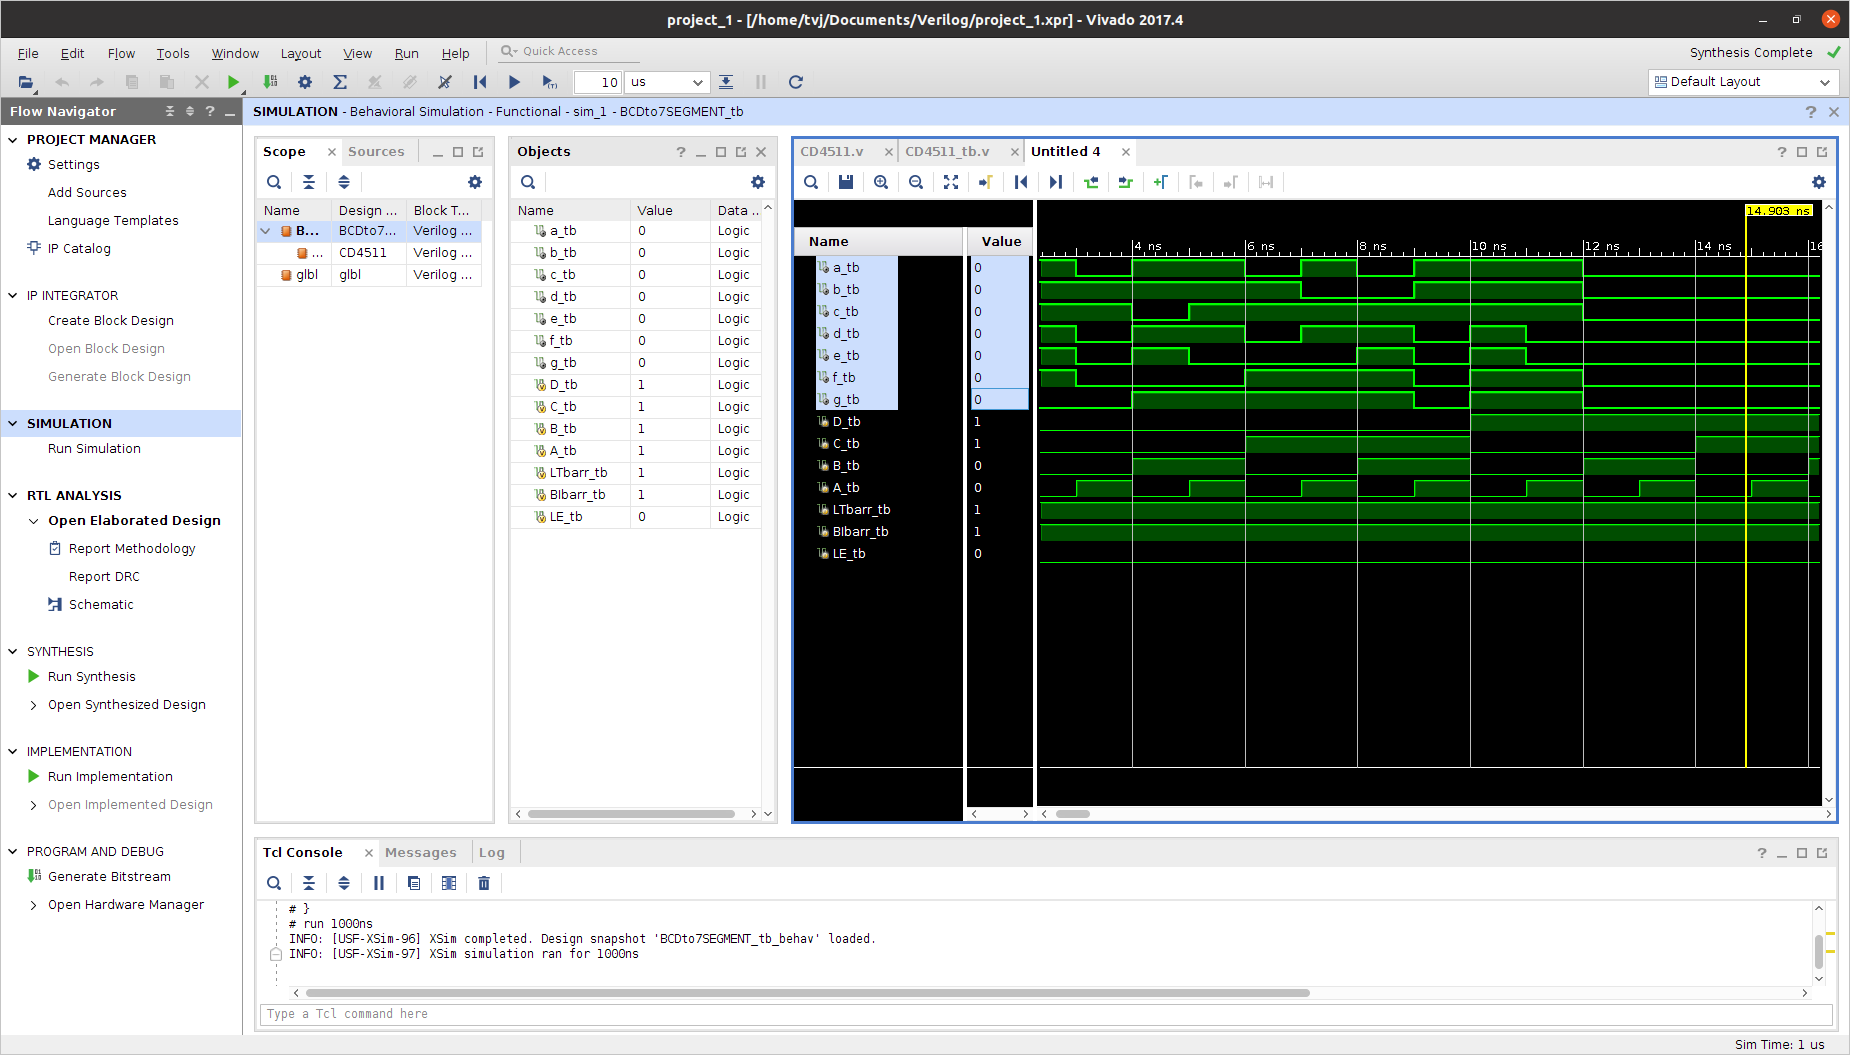
\includegraphics[width=\linewidth]{fig/vivado/3_simu.png}
                    \caption{CD4511的行为仿真}
                    \label{fig:vivado_3_simu}
                \end{figure}
    
                \begin{figure}[htbp]
                    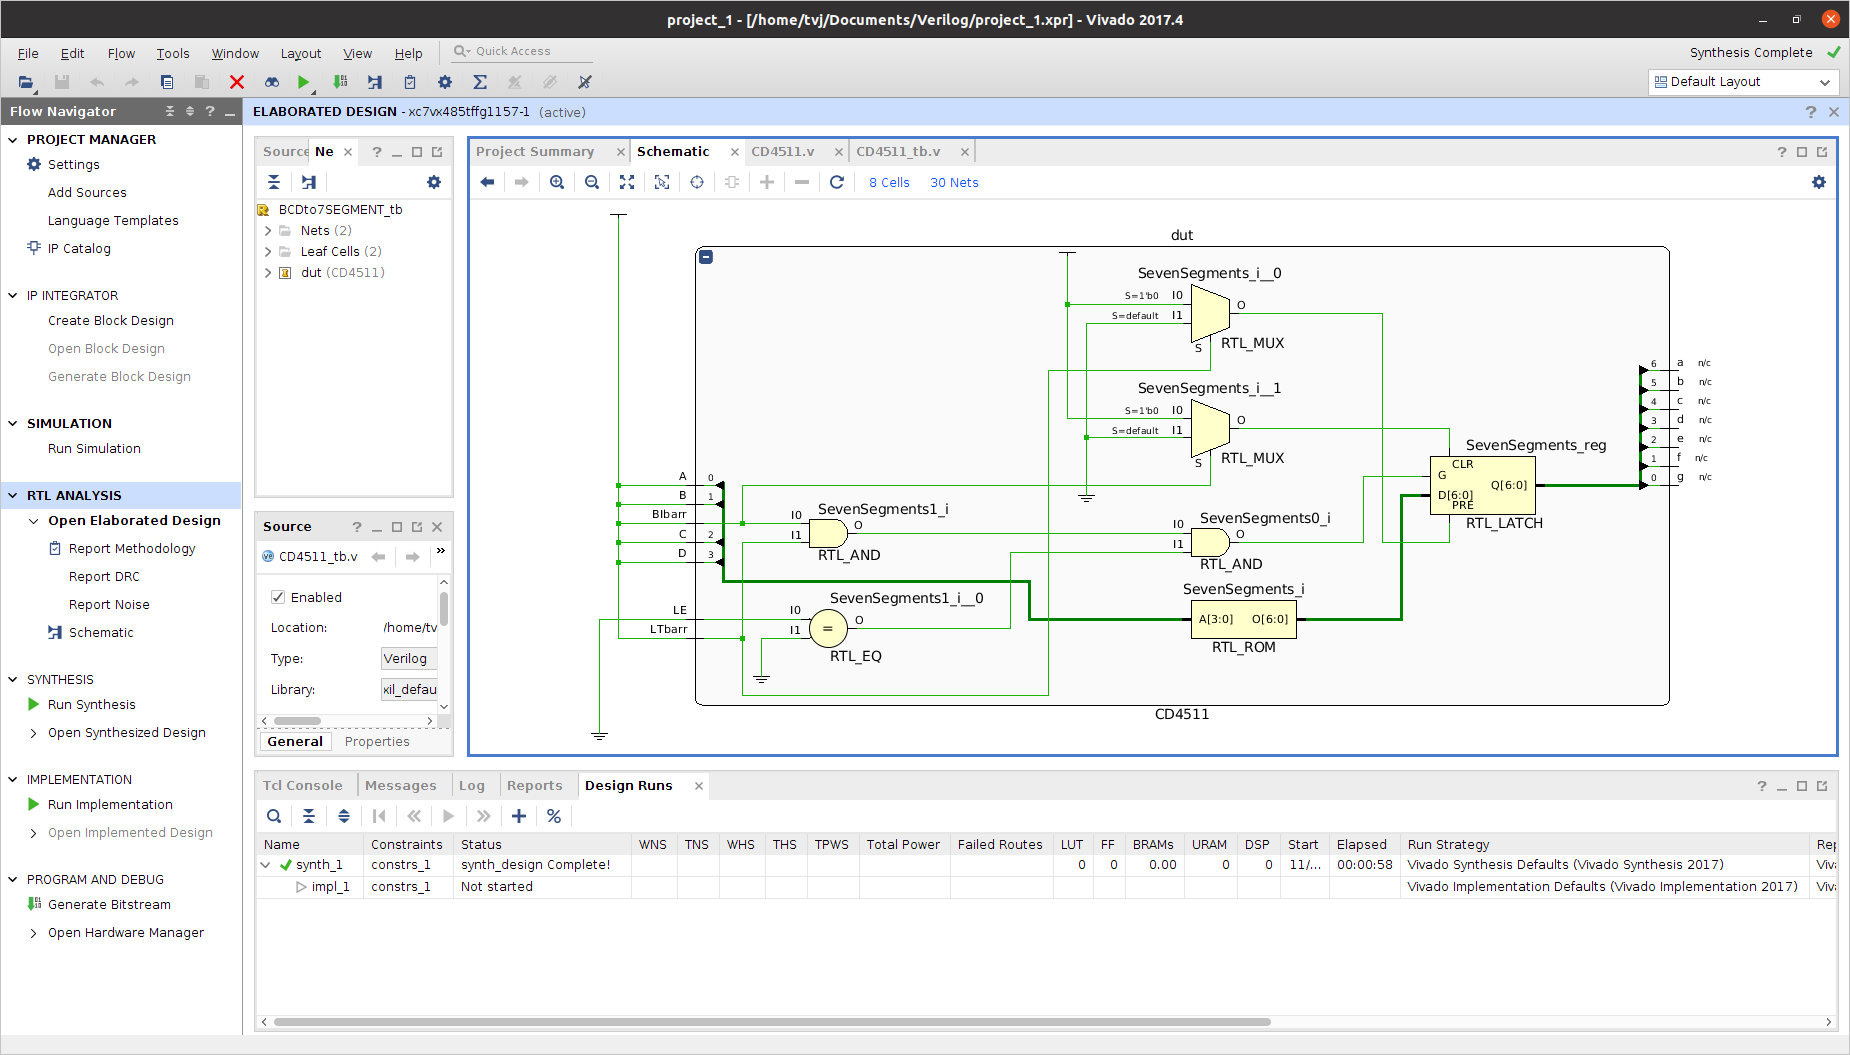
\includegraphics[width=\linewidth]{fig/vivado/3_RTL.png}
                    \caption{CD4511的RTL级电路}
                    \label{fig:vivado_3_RTL}
                \end{figure}
     
            \newpage
            \section{探索与应用设计}

            \subsection{环形振荡器电路}

            在图~\ref{fig:1_circuit}~的基础上增加一条导线,观察震荡电路.

            \begin{figure}[htbp]
                \centering
                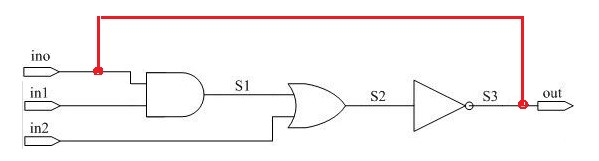
\includegraphics[width=.5\linewidth]{fig/3logic_.jpg}
                \caption{环形振荡器电路\cite{guide}}
                \label{fig:1_circuit_}
            \end{figure}

            在此处,取 $in_1=1, in_2=0$ 恒定.
            我自己设计得到了以下的代码:

            \begin{lstlisting}[language=verilog, title=cl01\_pro\_tb.v]
module cl01_pro_tb(input [2:0] in, output out1); // testbench file
  reg xin; // Only in0 works, while in1 as 1 and in2 as 0
  wire out;
  wire [2:0] s; 
  cl01_pro DUT(.in(xin),.S1(s[0]),.S2(s[1]), .S3(s[2]), .out(out)
  );

  assign out1=out;
  initial begin
    #1 xin=0;
  end
  always @ * begin
    xin=out; // feedback from S3 to in0
  end
endmodule
                \end{lstlisting}
                \begin{lstlisting}[language=verilog, title=cl01\_pro.v]
`timescale 1ns / 100ps 
module cl01_pro( 
  input in, // in0 only
  output S1,S2,S3,
  output out
); // GATE model
  // wire S0,S1,S2,S3;
  and #1 U1(S1,in,1); // in1=1
  or  #2 U2(S2,S1,0); // in2=0
  not #3 U3(S3,S2);
  assign out=S3;
endmodule
                \end{lstlisting}

                \begin{analyze}{}{}
                    代码主要是添加了 feedback,实现方法是使用了\texttt{always}语句,使得每一次进入\texttt{cl01\_pro}模块的输出结果 $out$ 返回给 $in_0$,由于门延时,形成了如图~\ref{fig:vivado_4_simu}~所示的震荡效果.
                    此外可以观察到,$S_{1,2,3}$ 中间存在相位差,就是一个门所造成的.
                \end{analyze}

                \begin{idea}{Vivado 实战遇到的问题}{}
                    在具体的操作中遇到了几个问题,现在在此记录下来,准备在未来不断的学习中逐渐找到感觉来解决.
                    \begin{itemize}
                        \item 对于模块的 \texttt{input} 做 \texttt{assign} 无效;
                        \item \texttt{inout} 类型编译错误.
                    \end{itemize}
                    我一直认为编程属于``熟能生巧''的工作,所以不太希望直接对着教程来一步一步走,而是在自己的探索中寻找到一种写代码的合理的感觉.
                    {
                        \kaishu
                        题外话:我目前在做 IRS 信道估计方向的研究时,
                        也没有先去了解对应的基础知识,而是在看论文的基础上对问题有了一个整体的认识,随后包括 \texttt{MATLAB},\texttt{Python} 等技巧就自然掌握了.
                    }
                \end{idea}

                \begin{figure}[htbp]
                    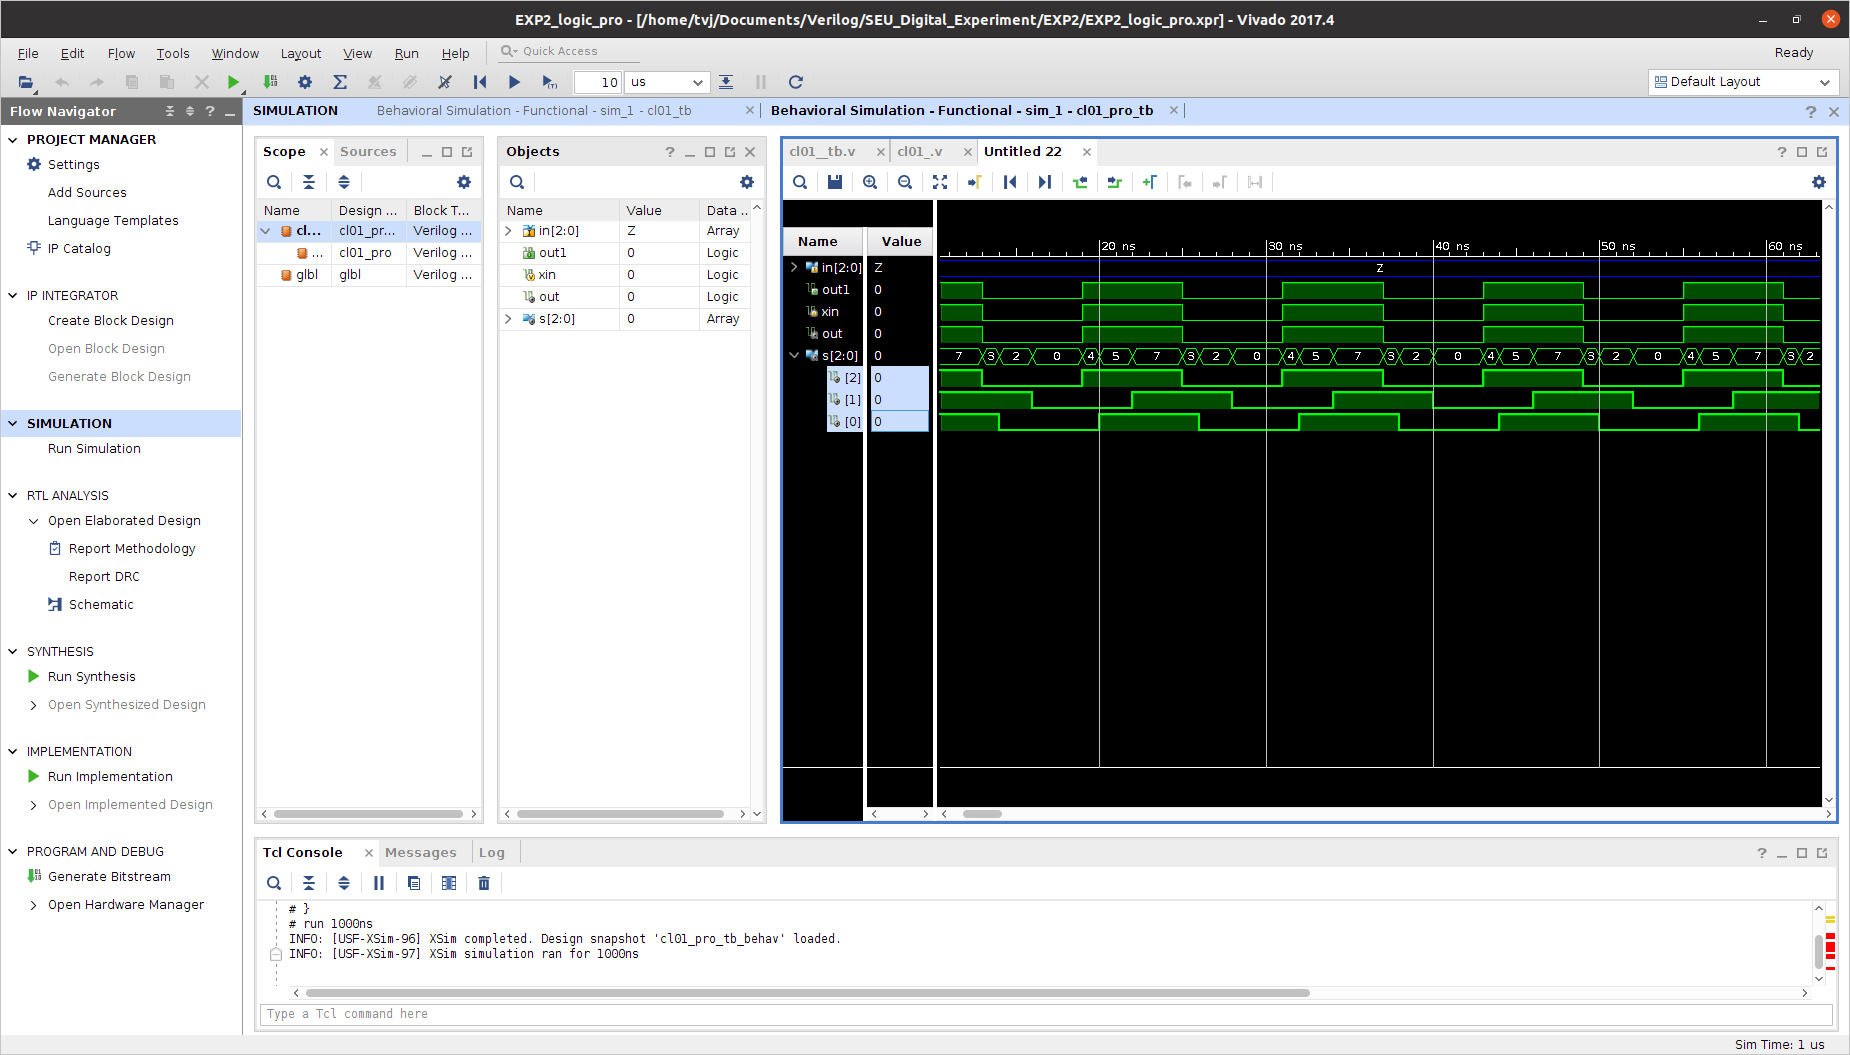
\includegraphics[width=\linewidth]{fig/vivado/4_simu.png}
                    \caption{环形震荡电路的行为仿真}
                    \label{fig:vivado_4_simu}
                \end{figure}
    
                \begin{figure}[htbp]
                    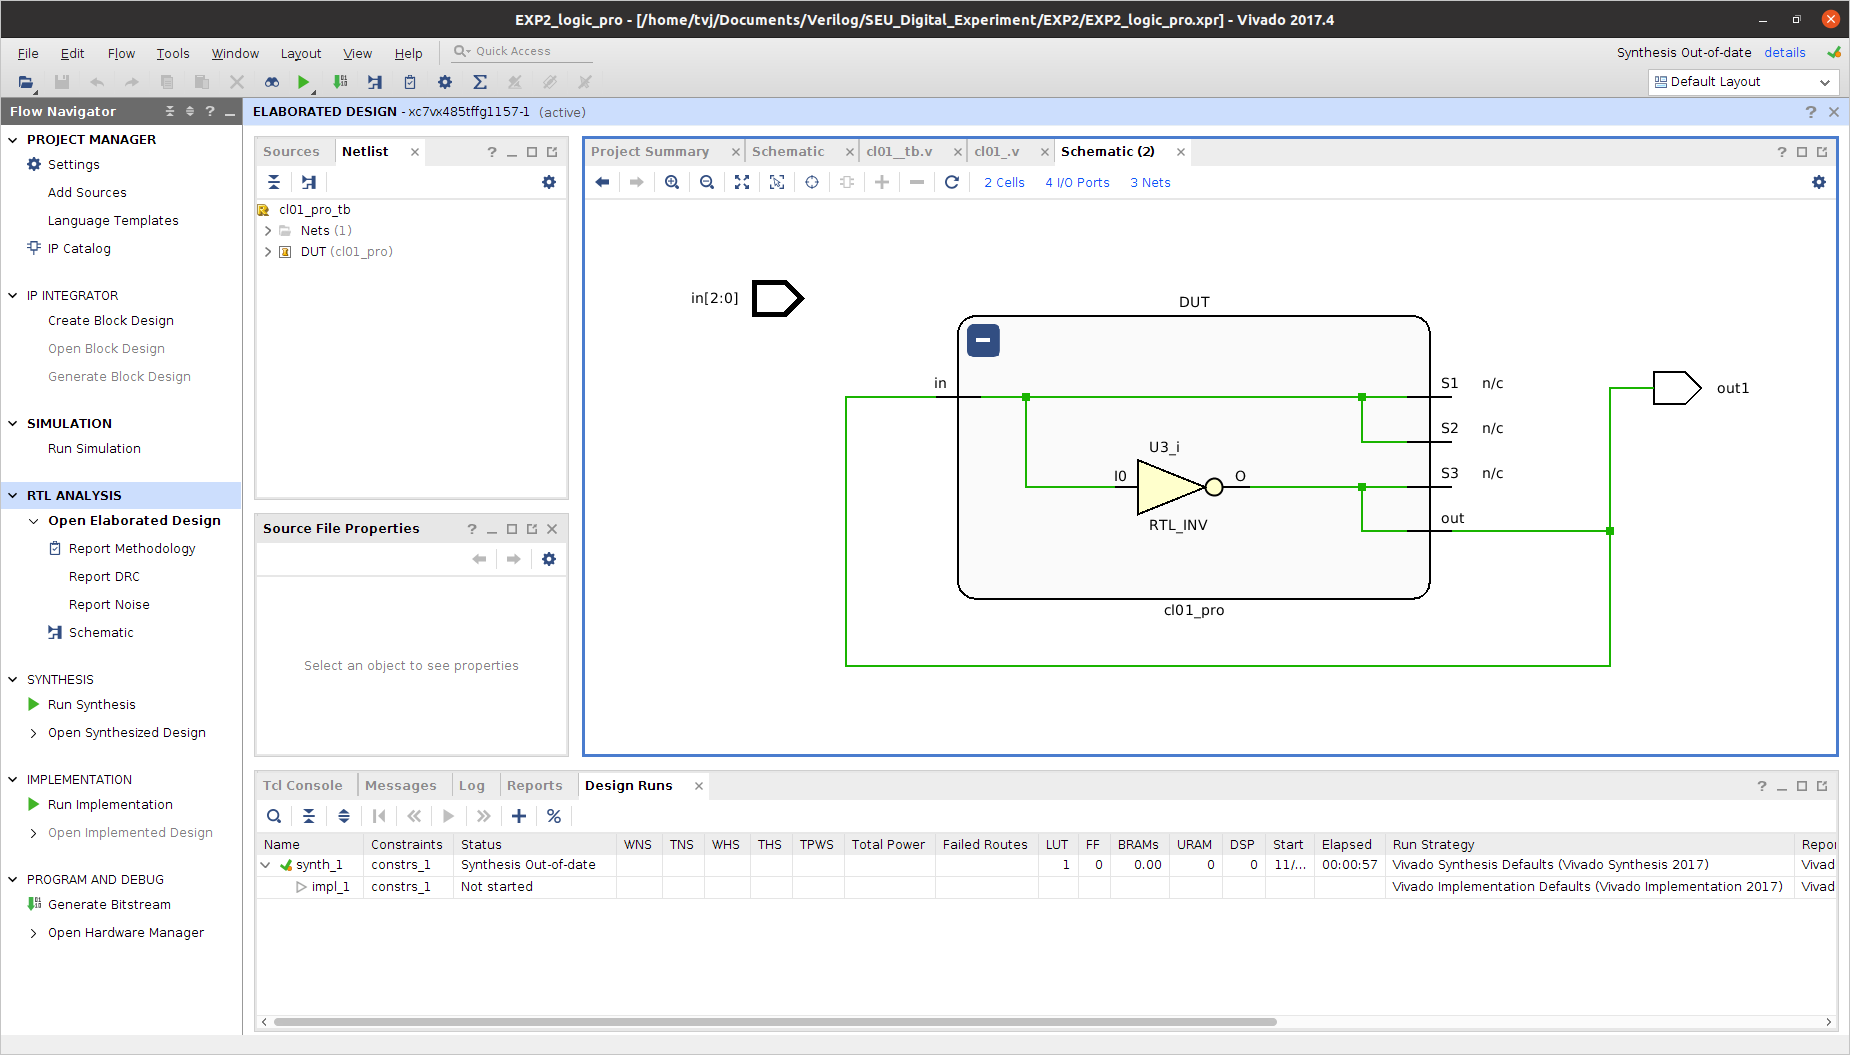
\includegraphics[width=\linewidth]{fig/vivado/4_RTL.png}
                    \caption{环形振荡电路的RTL级电路}
                    \label{fig:vivado_4_RTL}
                \end{figure}

            \newpage
            \subsection{选做实验实现分析}

            \begin{itemize}
                \item \textbf{复用器}:结构图简单,可以参见文献\cite{guide};转换更高位数时需要互相连接,总的来说就是嵌套,有主从(master-slave)结构的存在.
                \item \textbf{三态8 总线驱动器数据流}:具体实现较为简单,和之前在实验箱上完成的工作类似,都可以依据电路图完成.
            \end{itemize}

        \section{实验总结}

            硬件的实验总体来说较为简单,只需要将原理理解清楚后动手操作即可.
            这里也比较强调一些规范性,例如示波器要求共地、实验箱各个模块需要检验等等.

            Vivado 的实验我认为是比较有难度的,需要在整体上对于所写的内容要有一个较为深入的理解,然后就要熟悉 Verilog 的基本语法,通过代码描述出这个硬件.
            目前我所在的课题组内能将硬件做好的人不多,除了算法,我也需要在硬件上有一定的技术,这样能够有更加全面的发展,很多工作时需要有算法的硬件实现部分的.


    % 打印参考文献
    \addcontentsline{toc}{section}{参考文献}
    \printbibliography[sorting=none]

    \newpage
    \addcontentsline{toc}{section}{附录 A:实验报告 \LaTeX 模板}
    \section*{附录 A:实验报告 \LaTeX 模板}

        实验报告使用自己编写的 \LaTeX 模板(\texttt{SEU-Digital-Report.cls}),
        在基本适配 Microsoft Word 版报告的格式要求之外,
        增加了更多的功能,使得报告看起来更加优雅多彩.

        后续升级后,报告模板将于 \url{https://github.com/Teddy-van-Jerry/TVJ-Digital-Report} 基于 MIT License 开源共享.

        编译需要使用 \texttt{XeLaTeX + Biber},封面页修改如下内容即可.
        \begin{lstlisting}[
            language=tex,
            morekeywords={
                expno,
                expname,
                expauthor,
                expID,
                expmates,
                expmatesID,
                expmajor,
                explab,
                expdate,
                expreportdate,
                expgrade,
                exptutor,
                today
            }
        ]
%%%%%%%%%%%%%%%%%%%% 报告基本信息 %%%%%%%%%%%%%%%%%%%%
\expno{二} % 实验序号
\expname{组合逻辑与设计} % 实验名称
\expauthor{赵舞穹} % 姓名
\expID{61520522} % 学号
\expmates{郑瑞琪} % 同组
\expmatesID{61520523} % 学号(同组)
\expmajor{工科试验班} % 专业
\explab{计算机硬件技术} % 实验室
\expdate{2021年11月5日} % 实验日期
\expreportdate{\today} % 实验日期
\expgrade{} % 成绩评定
\exptutor{冯熳} % 评阅教师
%%%%%%%%%%%%%%%%%%%%%%%%%%%%%%%%%%%%%%%%%%%%%%%%%%%%
        \end{lstlisting}

    \addcontentsline{toc}{section}{附录 B:Vivado 程序真伪判别}
    \section*{附录 B:Vivado 程序真伪判别}

    \begin{enumerate}
        \item Vivado 程序我在 Ubuntu 20.4 LTS 平台完成,标题栏为经典的 GNOME 桌面风格,与 Windows 有很大区别.
        \item 标题栏现实程序所在文件夹为 \texttt{/home/tvj/Documents/Verilog/SEU\_Digital\_Experiment},这是我的 GitHub 私有项目.
    \end{enumerate}

\end{document}
